% This is samplepaper.tex, a sample chapter demonstrating the
% LLNCS macro package for Springer Computer Science proceedings;
% Version 2.21 of 2022/01/12
%
\documentclass[runningheads]{llncs}
%
\usepackage[T1]{fontenc}
\usepackage{float}
% T1 fonts will be used to generate the final print and online PDFs,
% so please use T1 fonts in your manuscript whenever possible.
% Other font encondings may result in incorrect characters.
%
\usepackage{graphicx}
% Used for displaying a sample figure. If possible, figure files should
% be included in EPS format.
%
% If you use the hyperref package, please uncomment the following two lines
% to display URLs in blue roman font according to Springer's eBook style:
%\usepackage{color}
%\renewcommand\UrlFont{\color{blue}\rmfamily}
%
\usepackage{listings}
\usepackage{verbatim}
% Used for making  comments. 
\usepackage{placeins}
% If you use a FloatBarrier to prevent figures sliding to unwanted sections.

\usepackage{todonotes}

\begin{document}
%
\title{Ontology-Based Models of Chatbots for Populating Knowledge Graphs}
%
%\titlerunning{Abbreviated paper title}
% If the paper title is too long for the running head, you can set
% an abbreviated paper title here
%
\author{Petko Rutesic\inst{1}\orcidID{0000-0001-7017-707X} \and
Dennis Pfisterer\inst{2}\orcidID{0000-0002-4877-1088} \and
Stefan Fischer\inst{2}\orcidID{0000-0003-1292-8925}}

%
\authorrunning{Rutesic et al.}
% First names are abbreviated in the running head.
% If there are more than two authors, 'et al.' is used.
%
\institute{Baden-Wuerttemberg Cooperative State University, 68163 Mannheim, Germany \and
  Institute of Telematics, University of Luebeck, Luebeck, Germany
}
%
\maketitle              % typeset the header of the contribution
%
\begin{abstract}
Knowledge graphs and graph databases are nowadays extensively used in various domains. However, the task of manually creating knowledge graphs using existing ontology concepts is quite challenging.  On the other hand, chatbots are one of the most prominent technologies in the recent past. In this paper we consider exploiting knowledge graphs as models of chatbots. These chatbots are to be used to populate knowledge graphs manually in a more convenient way. To implement chatbots we generate models which are ontology instances created using our proposed ontology as a meta-model. The models are exploited to generate chatbots which are in turn used by users to populate ontology instances of target (domain) ontologies. In this paper we consider generating graphs that model these chatbots. The approach that we propose here enables easier manual population of knowledge graphs using automatically generated conversational agents.
\keywords{modelling  \and ontology \and chatbots \and knowledge graphs}
\end{abstract}
%
%
%
\section{Introduction}

Creating user-friendly interfaces to facilitate populating knowledge graphs manually is a very demanding task. In order to create a knowledge graph, it is necessary to have expertise not only in the domain of interest but also in the field of ontology engineering. We can consider an example of flight registration where the end product would be a knowledge graph representing a particular flight. It should be selected an ontology for flight description and the user has to define an individual of a corresponding class that represents flights. Then the user has to know how to define departure and arrival airports. This requires the knowledge of object and data properties that can be used to describe those airports. What makes this task even more complex is to choose whether these destinations can be described as blank nodes or not. Creating these ontologies (editing RDF graphs) using only text editors in any syntax for representing RDF graphs would be intimidating for the majority of users.

Tools for ontology engineering like Protégé, WebProtégé, TopBraid Composer and similar tools are frequently used for this purpose. Additionally, there are many approaches to model user interfaces to populate knowledge graphs. These user interfaces are of different kind, from desktop and web-application to conversational agents (chatbots). In particular, chatbots have seen great growth in popularity, especially in the last couple of years with the appearance of large language models and tools like ChatGPT that use deep learning models to generate correct humanlike responses. Chatbots are nowadays integrated in various domains and have numerous applications such as e-customer care services, e-commerce systems, medical field, etc. Since there has been a range of different methods used to create chatbots and to model dialogs in various ways, it turns to be natural to use knowledge graphs (ontologies) to model chatbots. Our approach consists of enabling end users to create knowledge graphs like the above-mentioned flight knowledge graph in a simple manner. The chatbot should mostly ask simple questions like: ``What is the flight number?'', ``What is the flight destination?'', etc. The novelty of our idea lies in the automatic generation of chatbots from models that themselves are knowledge graphs. Following this approach, the design of our conversational agent models becomes the task of ontology experts, whereas the end users of the conversational agents would not necessarily need expert knowledge in ontologies. This way, the end user would be relieved from the burden of precisely knowing domain ontologies and the intricacies of ontology engineering.

Our approach could be simply expressed as two function. The first function is named modelling function and it describes the process of modelling chatbot dialogues (conversations) and at the same time modelling the structure of output knowledge graphs. The modelling function takes as input parameters a set of domain ontologies and our $OBOP$ ontology (Ontology for Ontology-based Ontology Population) (\url{http://purl.org/net/obop}) which is actually used for modelling and can be found on Github\footnote{\url{https://github.com/ontosoft/logic-interface/blob/main/ontology/obop.owl}}.
$$ f_{modelling}(DomainOntologies, OBOP) = ChatbotModel$$
The modelling process is the task for ontology designers and the output of this process is a $ChatbotModel$ which is a knowledge graph defined using concepts from $DomainOntologies$ and our $OBOP$ ontology. 
The second function represents the process of data acquisition, i.e., knowledge graph population. This process is actually the use of chatbot to enter data.
$$f_{acquisition}(ChatbotModel, EnteredData) = OutputKnowledgeGraph$$
The acquisition function takes a chatbot model and the data entered by the user as the input parameters. The output of the acquisition function is a wanted knowledge graph defined using only concepts from the domain ontologies (called $OutputKnowledgeGraph$). In this paper we describe main elements of the OBOP ontology that model different parts of chatbot conversations and present how the modeling function works for a simple use case. Additionally, we present the acquisition function through the usage of the model to populate a knowledge graph using a chatbot.      

Since the main goal is to simplify the population of knowledge graphs using conversational systems (chatbots), we have explored the idea of modeling these chatbots also within knowledge graphs. To leverage the reasoning capabilities of OWL ontologies and still to have good computational complexity, it is reasonable for the chatbot models to be represented, if possible, in the OWL Lite ontology class. Therefore, the goal of our approach can be boiled down to the following set of requirements:
\todo{Stefan: I suggest explaining why these are requirements. Otherwise, it looks random.}
\begin{enumerate}
\item
  The chatbot conversation and the structure of the output knowledge graph are both specified within the same knowledge graph (e.g. RDF file), representing a model.
\item
  Models are defined using a dedicated ontology designed for this purpose, serving as a meta-model for generating our models.
\item
The Meta-model comprises elements capable of modelling main program control structures, i.e., sequential, selection (branching) and iteration control structures. 
\end{enumerate}
\begin{comment}
The requirements to  this approach are that chatbot models should provide Turing completeness. Basic branching structures, loops has to be implemented in models. Models schould be general and therefore not tailored only for one domain, but applicable in arbitrary domains. Functionalities of chatbot modeling such as program flows should be modelled using knowldege graphs (ontology instances). Models are not overly complex for the implementation. In the next sections we explain how to implement these requirement..
\end{comment}

In the rest of the paper, we explain how we implement proposed requirements.
The rest of the paper is organized as follows: In the next section, it is presented a use case with the flight registrations, which is exploited in subsequent sections to explain our approach. Afterwards, it is explained the design of the OBOP ontology which is used to generate our chatbots. Each subsection describes specific workflows of the chatbot and how those workflows are modelled by entities of the OBOP ontology. Finally, the paper concludes with the contribution section.

\section{Use Case}

\todo{Stefan: I do not really understand the use case, because the description is too unstructured. I suggest describing the process step by step, possibly as an enumeration list which explains who does what in the process and what the final result is. It would be even better to have a process graphic which shows the relation of the different ontologies, chatbots etc.}

To demonstrate the applicability of our chatbot models, we introduce an example involving a chatbot designed to facilitate the definition of flights. One potential group of users who could benefit from this chatbot includes airline personnel responsible for registering new flights and services related to those flights. Assuming that these users need to create a knowledge graph for each flight, we can employ the GoodRelations ontology\cite{hepp2008goodrelations} and the Ticket ontology\footnote{\label{Ticket Ontology}http://purl.org/tio/ns}, which aligns with the GoodRelations ontology. The knowledge graph that our chatbot constructs here is already presented in the examples of how to use the Ticket ontology. In Figure~\ref{fig:usecase}, we provide a simplified graphical representation of this knowledge graph for better visualization. 

The primary objective of our chatbot use case is to simplify the process for end-users by posing straightforward questions, while the knowledge graph is generated seamlessly in the background using answers to those questions. The chatbot must have the capability to generate this knowledge graph and also to accommodate its extensions, such as adding the definition of additional ticket types if needed. By doing so, the chatbot determines the structure of the output ontology without explicitly asking the user to specify blank nodes, instances of specific ontology classes and other details, thereby alleviating the burden of detailed ontology engineering. To achieve this level of sophistication, the chatbot model incorporates all the necessary details, and the key aspects of the model are outlined in the section dedicated to modeling architecture.
\begin{figure}[H]
  \centering
  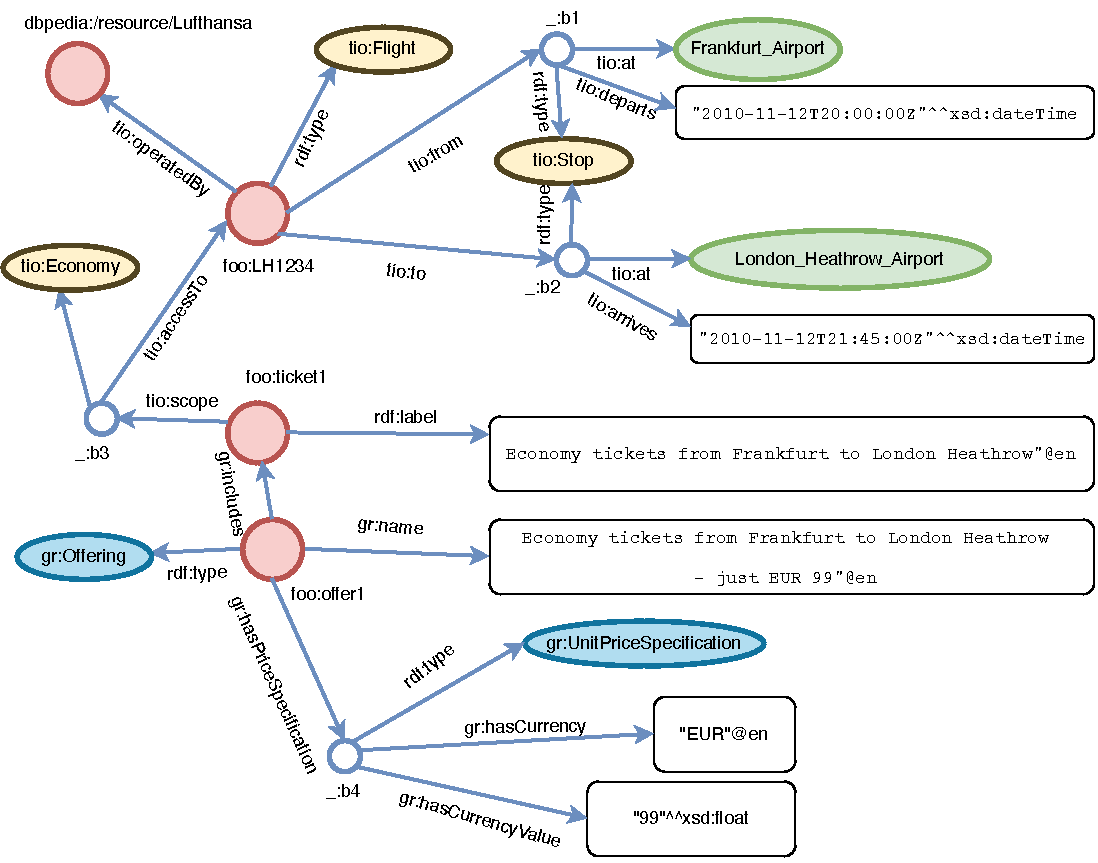
\includegraphics[width=\linewidth]{img/use_case}
  \caption{A knowledge graph representing a simple flight description.}
  % \Description{Big picture }
  \label{fig:usecase}
\end{figure}


The knowledge graph contains data about a specific flight with the flight number LH1234, which is operated by Lufthansa airline. The flight information includes details about the departure and destination airports, as well as the types of tickets that can be booked for that flight. A flight ticket is defined as an instance of the class tio:Ticket of the Ticket ontology. In the graphical representation, individuals and blank nodes are depicted using circles, with blank nodes represented by empty circles. Ontology classes are illustrated by ovals, while data properties are shown as rectangles. 

\FloatBarrier
During the interaction with the chatbot, the user must provide the flight number, departure and destination airports, as well as the departure and arrival times.
Below is a representation of the example knowledge graph in RDF format using Turtle syntax, with the prefix definitions omitted for brevity:
\begin{lstlisting}[basicstyle=\small]
foo:LH1234 a tio:Flight ;
  tio:from [ a tio:Stop ;
     tio:at <http://dbpedia.org/resource/Frankfurt_Airport> ;
     tio:departs "2010-11-12T20:00:00Z"^^xsd:dateTime ] ;
  tio:to [ a tio:Stop ;
     tio:at <http://dbpedia.org/resource/London_Heathrow_
       Airport> ;
     tio:arrives "2010-11-12T21:45:00Z"^^xsd:dateTime ] ;
  tio:availableServiceLevel tio:Economy, tio:BusinessClass ;          
  tio:operatedBy  <http://dbpedia.org/resource/Lufthansa> .
            
foo:ticket5 a tio:TicketPlaceholder ;
  rdfs:label "Economy tickets from Frankfurt to
       London Heathrow"@en ;
  tio:scope [ a tio:ScopeOfAccess ;
     tio:accessTo foo:LH1234 ;
     tio:eligibleServiceLevel tio:Economy ] .

foo:HeppTickets gr:offers foo:offer1 .
foo:offer1 a gr:Offering ;
     gr:name "Economy tickets from Frankfurt to London
          Heathrow - just EUR 99"@en ;
     gr:description "Special Offer: Economy tickets from
          Frankfurt to London Heathrow for just EUR 99"@en ;
     gr:includes foo:ticket5 ;
     gr:eligibleRegions "DE"^^xsd:string ;
     gr:hasBusinessFunction gr:Sell ;
     gr:hasPriceSpecification
       a gr:UnitPriceSpecification ;
         gr:hasCurrency "EUR"@en ;
         gr:hasCurrencyValue "99"^^xsd:float ;
         gr:validThrough "2010-11-11T23:59:59"^^xsd:dateTime];
     gr:acceptedPaymentMethods gr:MasterCard, gr:VISA ;
     gr:availableDeliveryMethods tio:Etix .	
\end{lstlisting}
The knowledge graphs (instances of the Ticket ontology) generated using our chatbot offer significant usefulness as they can be easily searched by customers looking to book flight tickets. The use of ontologies in the system allows for defining search operations using SPARQL queries.
Moreover, customers have the option to employ conversational agents like KBot\cite{ait2020kbot} in order to find suitable flight tickets using natural language understanding over linked data. In that case semantic web technologies can be used directly to find suitable flights without resorting to web scraping methods as described in \cite{turnip2019application}.        
   
\section{Related work}
One of the first known conversational agents is ALICE \cite{wallace2009anatomy} which uses AIML (Artificial Intelligence Markup Language) which is basically XML to design conversations. The system uses a botmaster which monitors conversations to make them more appropriate. Unlike writing rules in a XML based language, the rules in our approach are encoded in an ontology instance and can be stored in an RDF file. Historically, there have been different approaches as to how to use semantic nets to generate chatbot. One of the first examples is OntBot \cite{al2011ontbot} that transforms ontologies and knowledge into relational database and then uses relational database to generate chats. Another example of usage of model driven conversational systems is presented in \cite{perez2020model}, where a special domain-specific language with elements such as intents, entities, actions and flows is used to design the dialogue structure of task oriented chatbots. In contrast, our idea is to represent those elements such as intents and actions in knowledge graphs. \cite{bocklisch2017rasa}

There has been many approaches to model user interfaces and web-application logic using knowledge graphs. An approach described in ~\cite{rutesic2021enhanced} proposes a way of modelling of HTML application structure and its logic using RDF graphs.
In this paper we deal with the question of modeling and generating chatbots that are used to maintain dialogs with users to acquire data. Moreover, those acquired data are used to directly populate corresponding domain ontologies (knowledge graphs). The expressiveness of formal ontologies came into handy to represent both the models of chatbots and the complex knowledge in the business logic of target ontologies. According to \cite{agarwal2020review} conversational clients or chatbots are designed to be used either as task-oriented or open-ended dialog generators. In our approach we develop a task-oriented chatbot that has to collect data (ontology instance) of a particular ontology. The actual task is described based on rules specified in the model represented as an ontology instance defined using our OBOP ontology. Thus, our chatbot can also be classified as a rule-based chatbot. To enable humanlike conversation our task-based chatbot module is incorporated in a an open-ended chatbot which is further described in the implementation section.     

The intention of our system is not to design a chatbot capable of convincing a human that (s)he is chatting with a human instead of a computer program. That intelligent behavior depends on good knowledge sets. Conversely, we focus on the creation of chatbots that acquire information in the form of knowledge graph, which are individuals (instances) of the corresponding domain ontologies.  



\section{Model architecture}
Our meta-model (OBOP ontology) contains various structures that describe chatbot functionalities. The fundamental structure is designed to specify a simple data request. In response to this data request, the user is required to enter a value. The entered value is then validated and can be stored in the system as a data property, an IRI or for a similar purpose. This functionality corresponds to entering data in a form field in GUI interfaces. To represent inserting this data values, the OBOP ontology, uses an instance of the class obop:SingleValueRequest. In cases where multiple data properties need to be entered as a group of questions, then it is modeled using a conversation block.

\subsection{Conversation block}
A conversation block represents a part of conversation used to collect data values which are frequently related to a specific entity. This part of the dialog is analogous to a HTML form in web applications. The chatbot poses several questions and by entering answers to those questions, the system stores corresponding values. A simple model to enter the flight IRI is illustrated in Figure~\ref{fig:conv_block}. In this figure, blue circles represent instances of classes of the OBOP ontology, while slightly bigger circles in peach color represent instances of domain (target) ontologies, yellow ovals represent classes of the OBOP ontology and blue ovals stand for the target ontology classes. Object and data properties are denoted by directed lines with labels that specify names of those properties.     

\begin{figure}[H]
  \centering
  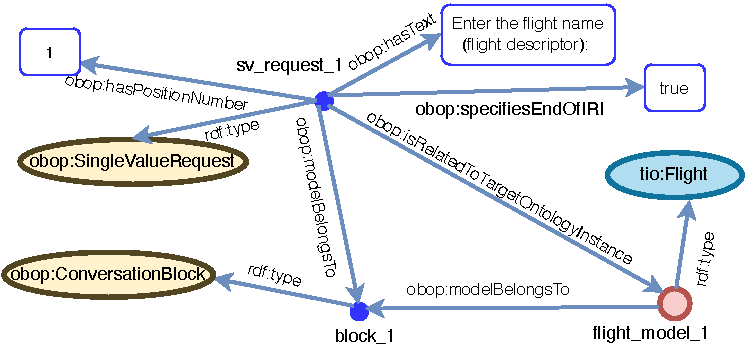
\includegraphics[width=\linewidth]{img/conversation_block}
  \caption{Modeling a block of conversation}
  % \Description{Modelling conversation block of the chatbot sytem }
  \label{fig:conv_block}
\end{figure}


A part of the model represented in the Figure ~\ref{fig:conv_block} should initiates the following conversation:
\begin{lstlisting}[basicstyle=\small,  xleftmargin=0.7cm ]
chatbot: Please enter the flight name (flight descriptor):
user:    LH1234
\end{lstlisting}
The result of this conversation will be the following tripple:
\begin{lstlisting}[basicstyle=\small,  xleftmargin=0.7cm ]
foo:LH1234 a tio:Flight. 
\end{lstlisting}
In Figure~\ref{fig:conv_block} can be seen a conversation block named \textit{block\_1} that  models a simple conversation containing one instance of the class obop:SingleValueRequest called \textit{sv\_request\_1} that represents a question for entering a flight name (unique flight descriptor). \textit{sv\_request\_1} has the object property obop:specifiesEndOfIRI which has a boolean values. The value true stipulates that the data entered as the answer to the question will be used as the end of IRI representing the instance of the flight. The model of the instance of tio:Flight class that will be generated in this process is represented by the \textit{flight\_model\_1} instance. During the conversation with the chatbot from this instance will be generated the instance with the name foo:LH1234. If the inserted string had to be value of some data property instead of part of the IRI then it would be specified by a \textit{obop:containsDatatype} object property of \textit{sv\_request} instance which would specify name of wanted data property. The object property \textit{obop:isRelatedToTargetOntologyInstance} indicates what instance will be transformed with the entered data. The data property \textit{obop:hasPositionNumber} specifies that this is the first question in this conversational block.  


\FloatBarrier
\subsection{Branching control structure}
To enable chatbot users to make decisions and select different paths of execution, the OBOP ontology has means to model branching control structures. The class \textit{obop:Branching} represents a conditional structure. A simple branching structure in our example is explained in the case of choosing an airline that operates the current flight. The chatbot user is therefore asked to choose exactly one airline company among those presented options.  
One possible conversation is presented in the following listing:
\begin{lstlisting}[basicstyle=\small,  xleftmargin=0.7cm ]
chatbot: Enter the airline that operates your flight.
         Choose one of the following options:
         1. Lufthansa
         2. Ryanair
user:    Lufthansa 
\end{lstlisting}
The chatbot asks a question and specifies a list of possible options. The user responds by writing one among those listed names or by writing the ordinary number in front of the corresponding name. For the sake of brevity, we decided to present only two possible options (two airlines) to choose from. This statement is similar to the ''switch'' statement in programming languages. As the result of the execution of this part of the chatbot the output graph can be extended with the following triple:
\begin{lstlisting}[basicstyle=\small,  xleftmargin=0.7cm ]
foo:LH1234
  tio:operatedBy <http://dbpedia.org/resource/Lufthansa>.
\end{lstlisting}
The part of the model that generates the previous chatbot question and adds the specified triple, as the consequence of the chosen option, is represented in Figure \ref{fig:branching_schema}. It can be seen that the same conversational block \textit{block\_1} is used because we consider it as the part of the same conversation section. The question to choose one of multiple possible values is denoted by the instance of the class obop:Question called \textit{question\_1}. \textit{question\_1} has the data property \textit{obop:hasTex} with the text of the question. Additionally, the question has the value 2 of the \textit{obop:hasPositionNumber} data property that serves to denote that this question has second place in the conversation block.         
The question \textit{question\_1} has an instance of the class \textit{obop:hasBranching} called \textit{branching\_1} and this branching is specified by the instance of the \textit{obop:Connection} class named \textit{conn\_1}.
\begin{figure}[H]
  \centering
  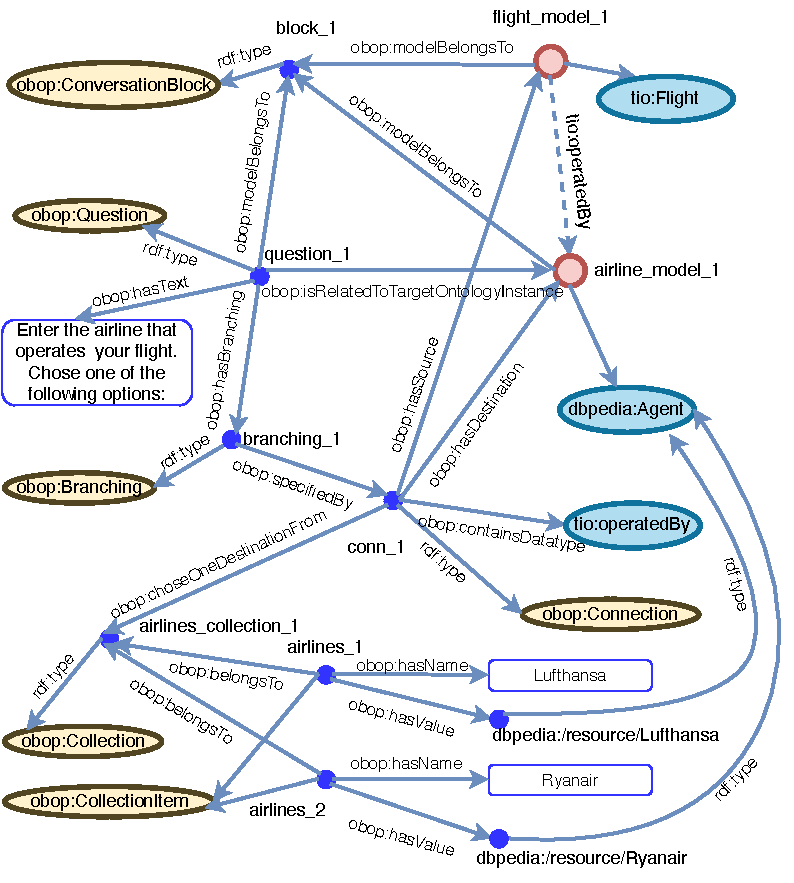
\includegraphics[width=\linewidth]{img/branching_schema}
  \caption{A part of the model specifying choosing of the airline.}
  % \Description{Branching to decide on the operating airline}
  \label{fig:branching_schema}
\end{figure}

The connection class specifies how the two instances of the ontology classes should be related. The instance of this class has functional properties that specify source and destination of object properties. In our case the source is \textit{flight\_model\_1} and the destination is \textit{airline\_model\_1} which serves as a model for an instace of the class \textit{dbpedia:Agent} that will be created during the chatbot execution. Additionally, the object property that has to be inserted in the output graph between these two instances is specified by the \textit{obop:containsDatatype} object property and it is in our case \textit{tio:operatedBy} property. This object property that has to be created is denoted by dashed line in Figure \ref{fig:branching_schema}. However, this edge is not part of the actual model graph.    

It can be seen that the connection instance specifies a predicate (object property) and an object (the instance) of a new triple. For our knowledge graph, the user needs to choose exactly one airline from the set of possible airlines. Another possibility would be to enable the user to simply type in an IRI of the wanted airline which has to be an instance of the class \textit{dbpedia:Agent}. Choosing an option from the list of available options would be mostly easier for the end user and we described that way. At the bottom part of the Figure \ref{fig:branching_schema} is defined an instance of the \textit{obop:Collection}class named \textit{airlines\_collection\_1}. The connection instance conn\_1 is related to this collection by the object property \textit{obop:choseOneDestinationFrom} which specifies exactly how to form the object of a new triple. In this case our simple collection contains two instances of the class \textit{obop:CollectionItem} corresponding to Lufthansa and Ryanair airlines. 
In order to stay in the scope of OWL Lite sublanguage, OBOP collections are not defined using rdf:Bag, rdf:Seq or by using restrictions like \textit{owl:someValuesFrom}. Collections are basically used by the chatbot program in the runtime phase and they are not used in the process of reasoning.     


\FloatBarrier 
\subsection {Iteration control structure}
To provide Turing completeness, the chatbot model has to provide definition of iteration structurues (loops). As the iteration structure in programming languages enables repeated execution of a specific block of code, iteration structure in chatbot enables repeating a set of questions of a conversation block or other activities. For this purpose OBOP ontology has a class \textit{obop:Loop}. 

The example of iterations can be presented in our example with flight tickets. The user has to define more different tickets types for the flight could lead the following conversation:
\begin{lstlisting}[basicstyle=\small,  xleftmargin=0.7cm ]
chatbot: Do you want to define one more ticket type?
user:    Yes
chatbot: Please enter the label of the ticket?
user:    Economy tickets from Frankfurt to London Heathrow
chatbot: Choose the service level of the ticket?
user:    Economy
chatbot: Do you want to define one more ticket type?
\end{lstlisting}
The result of executing the previous chatbot conversation is the following part of the graph:
\begin{lstlisting}[basicstyle=\small,  xleftmargin=0.7cm ]
foo:ticket5 a tio:TicketPlaceholder ;
  rdfs:label "Economy tickets from Frankfurt to London
             Heathrow"@en ;
  tio:scope [ a tio:ScopeOfAccess ;
     tio:accessTo foo:LH1234 ;
     tio:eligibleServiceLevel tio:Economy ] .
\end{lstlisting}
The part of the model that generates the previous part of chatbot conversation is illustrated in Figure \ref{fig:iteration_example}. The question \textit{question\_2} to ask for a new ticket type is related to an instance of the \textit{obop:Loop} class called \textit{loop\_1}. Each iteration of the loop specifies adding a new ticket which is represented by a conversational block \textit{block\_3}. If the user answers positively to the chatbot's question, a new ticket instance is generated according to the \textit{ticket\_model\_1}. Together with the ticket is generated a blank node corresponding to the \textit{\_:bnode} instance. The new blank node is related to the flight instance which is already created in the previous examples according to the \textit{flight\_model\_1}. The object properties \textit{tio:scope} and \textit{tio:accessTo} are also automatically created. However, \textit{rdf:label} had to be specified using \textit{obop:containsDatatype} object property. In order to choose between possible service classes (e.g., Business or Economy) a new question (\textit{question\_3}) and connection (\textit{conn\_2}) was necessary. \textit{conn\_2} is not completely presented and ontology classes of same instances are omitted in Figure \ref{fig:iteration_example} for the sake of easier readability.
\begin{figure}[H]
  \centering
  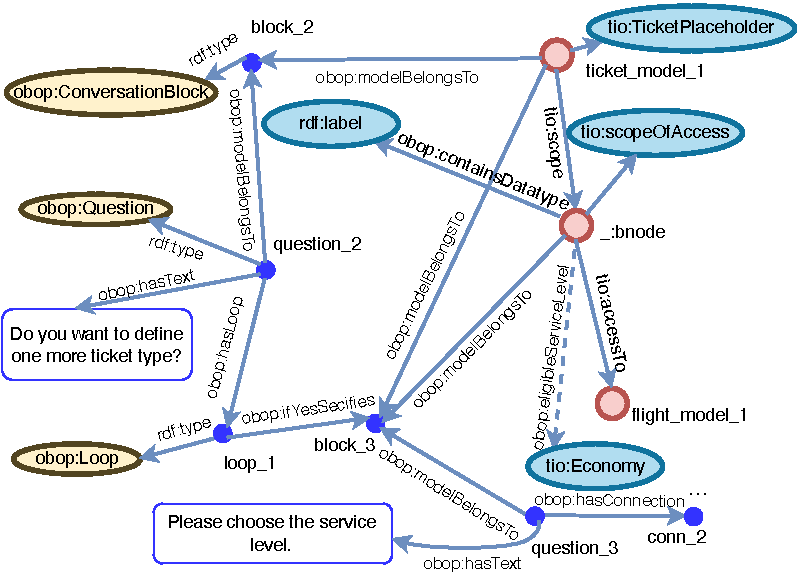
\includegraphics[width=\linewidth]{img/iteration_example}
  \caption{A part of the model that to define tickets using iteration.}
  % \Description{Iteration}
  \label{fig:iteration_example}
\end{figure}


\FloatBarrier 
\section {Implementation}

To implement a prototype of our chatbot, it was used a Python library called ChatterBot. To create and manipulate OWL ontologies is used a Python library for ontology-oriented programming Owlready \cite{lamy2017owlready}. The chatbot prototype can be tested as a REST application implemented using Flask framework\footnote{\label{flaskfootnote}https://flask.palletsprojects.com} with a simple JavaScript frontend. The source code can be found on Github\footnote{\url{https://github.com/ontosoft/ontochatbot}}. 

Chatbots generated using the ChatterBot library answer to the user questions based on functionalities of logic adapters. In that way, there is a time adapter to answer question such as `` What time is it?'', a math adapter that can respond to a request that requires an arithmetic operation, etc. When the user submits a question, all logic adapters check whether they can give response to that question or not. The ability of a logical adapter to answer the question is measured by the confidence factor which is expressed as the decimal value between 0 and 1. The answer from an adapter that has the highest confidence is chosen to be given as a reply. The architecture of our chatbot is shown in Figure~\ref{fig:architecture}.

\begin{figure}[H]
  \centering
  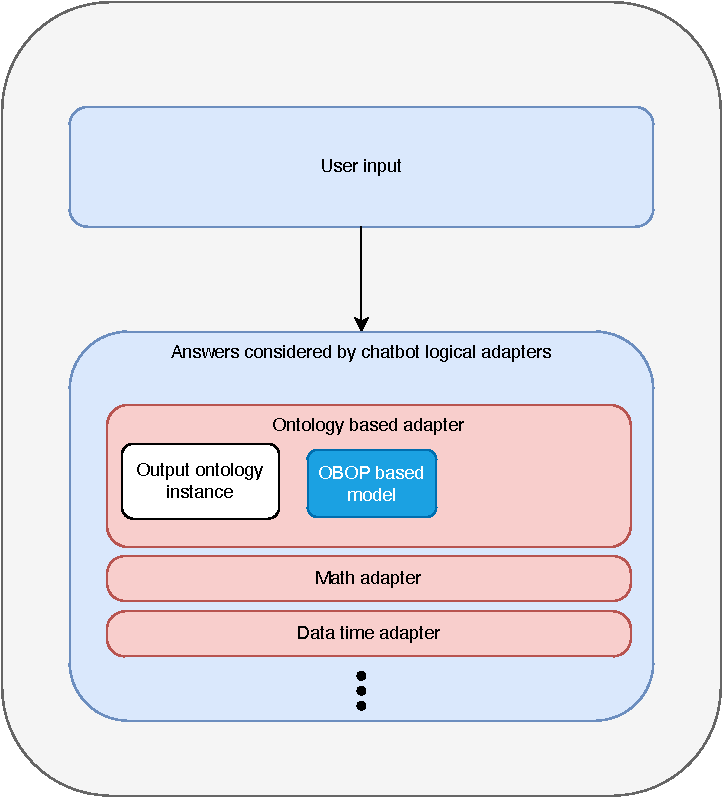
\includegraphics[width=0.5\linewidth]{img/architecture}
  \caption{Architecture of the chatbot system.}
  % \Description{Architecture o fthe chatbot sytem }
  \label{fig:architecture}
\end{figure}



Our model-based chatbot functionalities are implemented as a logic adapter for the ChatterBot library, namely it is called \textit{OntoBasedAdapter}. Unlike other chatterbot's logic adapters, OntoBasedAdapter keeps track of the current state of conversation. The conversation can be defined as $S=(C,\ (B1,U1,C2,U2,\dots))$. Letters B and U can be either question or answer and each of them could comprise of more sentences. Once the OntoBasedAdapter starts to gather information and populate the corresponding domain ontology, it must store information of the current state of the conversation. It is important to keep track of visited nodes and in this way enable system to make reverse steps and undo entering same data. Chatbot stores information on current context which is comprised of the entire array of nodes that have been visited and created during in the conversation till the current state. 

Keeping track of the state of the current dialogue is quite challenging task. 
In the paper ~\cite{altinok2018ontology}, authors dealt with this problem by exploiting ontologies as both knowledge base and for the dialog manager (domain-driven conversation). They used ontology-based dialog management to create a banking chatbot. Our chatbot is domain independent conversational client and domain is basically specified in the corresponding chatbot model. Yet another example of using knowledge based chatbot which is defined over link data is represented in \cite{ait2020kbot}.


\subsubsection{Answering questions and generating replies}
Once the OntoBasedAdapter takes charge of the dialog, it maintains the status of that conversation. The system asks questions in the order that is defined by the chatbot model. If the user asks a question which is not related to the current task specified in the model and the dialog takes other direction then can happen that another logic adapter can take over the charge and respond in order to make the conversation more lifelike. Subsequently, it is posed a question by OntoBasedAdapter to pick up the conversation at the very same point where it was interrupted. This is possible because the OntoBasedAdapter takes care of the context and the state of conversation.   
The confidence factor determines what logic adapter among all logical adapters will be chosen to give the answer. However, if the OntoBasedAdapter already started to gather information according to a conversation model then it has precedence over other logical adapters. Even though the user can abruptly change the subject of the conversation, the conversation agent tries to get the conversation back to the wanted topic. It could happen that the user asks ``What time is it?'' in the middle of the conversation that should schedule the flight details. In that case, the system answers the question using the \textit{Time logic adapter} and after that instantly asks the next question where it left off according to the chatbot model.

In this way each response is assigned with a corresponding weight (confidence factor). The challenges associated to this way of choosing replies include the fact that confidence factors of already implemented adapters tend to be quite high values. The other way is that OntoBasedAdapter always returns confidence factor equal to 1 after it started to collect information.  
Responses are hard-coded in the model by the model developer.




\section{Contribution}
In this paper we introduced models of conversational agents (chatbots) that can accomplish domain specific orders such as generation of flight descriptions, booking flight tickets or creation of restaurant menues that could be used for restaurant reservations in a simpler way for end users. 
In order to show how to create a chatbot model we designed a chatbot used for flight description.
Proposed chatbots follow the rule-based method of chatbots, replies are generated using rules which are intgerated in the models of corresponding conversations. These conversation models represent templates according to which replies (or questions) are created.   

The requirements to the approach which are specified in the introduction of the paper are fulfilled with our implementation. The conversation model and the structure of the knowledge graph are both included in the same knowledge graph according to the first requirement. The limitations of this approach are high complexity of the model graphs and challenging maintenance of the generated graphs. Second and third requirement are fulfilled by defining particular classes, object and data properties in the OBOP ontology which correspond to the basic programming control structures. 

\begin{comment}
  
The user has an aim to get an information and to accomplish a goal. In our case the ontology model is used to conclude what the chatbot should say next. 
Chatscript can use Wordnet ontologies to improve responses.

OpenCyc [20] and Wordnet [21] 

We start presenting the review of literature that considers using ontologies and chatbots. 

An example which illustrates how our modelling works is a definition of a simple flight itinerary for a flight booking. \verb|https://www.chegg.com/homework-help/questions-and-answers/flight-ontology-online-travel-portal-engaged-well-known-airline-develop-ontology-support-i-q86451860| 
\end{comment}

%
% ---- Bibliography ----
%
% BibTeX users should specify bibliography style 'splncs04'.
% References will then be sorted and formatted in the correct style.
%
\bibliographystyle{splncs04}
\bibliography{mybibliography}
%
\end{document}
